% =========================================================================
%  Biological Penalty Sharpness Bounds the Value of In-Season Replanning
%  in Multi-Field Hybrid Maize Seed Production
%
%  NOTE ON FORMAT: this file reproduces IEEEtran conference style using the
%  standard article class, so it compiles without IEEEtran.cls installed.
%  Conventions follow the supplied reference paper: full-width roman title,
%  a grid of author blocks, bold abstract and index terms with run-in italic
%  labels, centred small-caps section headings, "TABLE N" plus a small-caps
%  caption set ABOVE each table, and "Fig. N." captions set BELOW figures.
%  To submit, drop the body into the conference's official IEEEtran template.
% =========================================================================
\documentclass[10pt,twocolumn]{article}

\usepackage[letterpaper,top=0.75in,bottom=1.0in,left=0.625in,right=0.625in,
            columnsep=0.25in]{geometry}
\usepackage{times}
\usepackage{amsmath,amssymb}
\usepackage{graphicx}
\usepackage{booktabs}
\usepackage{algorithm}
\usepackage{algorithmic}
\usepackage[hidelinks]{hyperref}
\usepackage[labelsep=period]{caption}
\usepackage{titlesec}
\usepackage{balance}

\setlength{\parindent}{1em}
\setlength{\abovedisplayskip}{4pt}
\setlength{\belowdisplayskip}{4pt}

% ---- section headings: centred, small caps, Roman numerals -------------
\renewcommand{\thesection}{\Roman{section}}
\renewcommand{\thesubsection}{\Alph{subsection}}
\renewcommand{\thesubsubsection}{\arabic{subsubsection}}

\titleformat{\section}[block]
  {\normalfont\normalsize\centering\scshape}{\thesection.\quad}{0em}{}
\titlespacing*{\section}{0pt}{10pt plus 2pt minus 2pt}{6pt}

\titleformat{\subsection}[block]
  {\normalfont\normalsize\itshape}{\thesubsection.}{0.6em}{}
\titlespacing*{\subsection}{0pt}{8pt plus 1pt minus 1pt}{4pt}

\titleformat{\subsubsection}[runin]
  {\normalfont\normalsize\itshape}{\thesubsubsection)}{0.5em}{}[:]
\titlespacing*{\subsubsection}{\parindent}{4pt}{0.5em}

% ---- captions: tables above in small caps, figures below ---------------
\captionsetup[table]{position=top,labelsep=newline,justification=centering,
                     font=sc,labelfont=sc,skip=3pt,textformat=simple}
\captionsetup[figure]{position=bottom,font=small,labelfont=normalfont,
                      labelsep=period,skip=5pt,justification=justified}
\renewcommand{\tablename}{Table}
\renewcommand{\thetable}{\Roman{table}}
\renewcommand{\figurename}{Fig}

% ---- IEEE-style run-in abstract (no centred heading, no extra margins) --
\renewenvironment{abstract}
  {\small\bfseries\noindent\textit{Abstract}---\ignorespaces}
  {\par}

\newcommand{\TSI}{\mathrm{TSI}}
\newcommand{\EVPI}{\mathrm{EVPI}}
\newcommand{\VSS}{\mathrm{VSS}}

% ---- title block -------------------------------------------------------
\title{\vspace{-2.2em}\normalfont\LARGE
Optimised Sowing Scheduling for Multi-Field\\
Hybrid Maize Seed Production under\\
Anthesis-Synchrony Constraints}

% Four authors, set as a 2x2 grid. The department name is long, so a single
% row of four would crush each column; the grid keeps the lines unbroken.
\newcommand{\authblock}[2]{%
  \begin{minipage}[t]{0.43\textwidth}\centering
  \normalsize #1\\[2pt]
  \small Dept. of CSE in IoT, Cybersecurity including Blockchain\\
  \small Dayananda Sagar Academy of Technology and Management\\
  \small Bengaluru, India\\
  \small #2
  \end{minipage}}

\author{%
  \begin{tabular}{@{}c@{\hspace{3em}}c@{}}
  \authblock{C. Tejas}{tejasshekar29@outlook.com} &
  \authblock{Mayur Adiga}{adigamayur@gmail.com} \\[14pt]
  \authblock{Pavan Kumar Nayak}{nayakpavan0099@gmail.com} &
  \authblock{Kishore Kumar N.~H.}{kishorekumarrnh05@gmail.com}
  \end{tabular}}

\date{}

\begin{document}
\twocolumn[
  \begin{@twocolumnfalse}
  \maketitle
  \vspace{-1.0em}
  \end{@twocolumnfalse}
]
\begin{abstract}
\small\bfseries
Hybrid maize seed is produced on many isolated contract fields, but the two parent lines are sown by one supervised crew, and the day a field is sown sets the flowering dates of both parents and hence whether their pollen and silk windows overlap at all. Deciding which field the crew starts on which day is today done by hand. We formulate it as a two-stage stochastic scheduling problem coupling a shared sowing crew to parent-specific flowering synchrony, solve it exactly, score it with a published measured yield response, take flowering dates from CERES-Maize, and evaluate on twenty-one observed seasons at an Indian seed-production site. Against current practice --- correct per-hybrid offsets, fields taken in order --- the optimised assignment yields $+11.9$\% more seed overall and $+38$\% at the largest farm tested, because naive sequencing saturates at about 39 fields however many are offered while the optimised plan keeps placing them. Revising the plan in-season adds a further $+2.26$\% on average, and we show this depends on two quantities a producer can compute before writing software: it rises with the curvature of the yield penalty, from $+0.49$\% at a flat response --- where we reproduce the irrigation literature's finding that in-season adaptation adds little --- to $+9.14$\% at a sharp one, and it vanishes where crew capacity exactly matches demand. Model biology is validated against CIMMYT's published sowing intervals for six tropical hybrids, reproduced to within 1.5~days from data that played no part in building it. Code, weather, crop-model table and results are released.
\end{abstract}

\vspace{2pt}
\noindent{\small\textit{\textbf{Index Terms}}\textbf{---precision agriculture,
hybrid seed production, anthesis synchrony, sowing scheduling, decision
support, stochastic programming, rolling-horizon optimisation.}}
\vspace{6pt}

% =========================================================================
\section{Introduction}
% =========================================================================

\subsection{The operation}

Hybrid maize seed is produced by sowing two inbred parent lines --- a male
and a female --- in alternating rows on the same field, so that the female
is pollinated only by the male. The seed company contracts the fields to
growers, but the sowing itself is done by the company's own supervised crew,
because the row pattern and the timing of the two parents are what make the
product and are not left to the grower~\cite{chassaigne2021,chassaigne2020}.
A producer in a seed-growing belt therefore runs many isolated fields with
very few sowing units, each of which can start only a few fields in a day.

The two parents rarely flower at the same time if sown together, so the
agronomic literature supplies, for each parent pair, a recommended
\emph{sowing offset}: the number of days the male should be sown before or
after the female so that pollen shed coincides with silk
receptivity~\cite{marahatta2025,chassaigne2021,asefa2024}. Practitioners call
this \emph{nicking}. Maize pollen stays viable for 18--24 hours and the stigma
is receptive for two to three days~\cite{marahatta2025}. If the windows miss,
no seed forms: field experiments report seed yield falling 29--57\% as the
tasseling--silking interval (TSI) widens~\cite{marahatta2025}.

\subsection{What the supervisor decides, and why it is hard}

With the offsets in hand, someone still has to decide \emph{which field the
crew starts on which day}. Today that decision is made by the field
supervisor, by hand, with a degree-day table and a calendar: fields are
taken in the order they come, each started on the first day the crew is
free, with its recommended offset applied. The agronomic recommendations
are derived for a single field and then assumed to be deliverable; the one
study that states the assumption explicitly notes that ``it is assumed that
machinery is available to do the sowing, or, in the case of rains after the
first sowing, staff are available''~\cite{chassaigne2021}. We have not
surveyed producers, and we describe current practice as the literature and
its stated operational assumption describe it; Section~\ref{sec:limits}
records this.

Three things make the hand decision harder than it looks.
\emph{First, the fields compete.} A crew that can start $K$ fields a day,
with $N$ fields needing three visits each inside a sowing window of $T$
days, is saturated once $3N \ge TK$; past that point every field placed
early is another field placed late or not at all.
\emph{Second, the day a field is started sets its biology.} Flowering is
driven by accumulated thermal time, so a field started a week later flowers
in different weather, and the offset that synchronised its parents at the
planned date may not synchronise them at the actual one.
\emph{Third, rain closes fields.} A wet day makes a field untrafficable for
one to three days depending on its drainage, pushing its visit --- and every
visit queued behind it --- later. The supervisor is therefore juggling
$N$ fields, $T$ days, around fifteen candidate offsets per field, a crew
limit that couples every choice to every other, and weather that will not
be known until after the choices are made.

No existing tool addresses this decision (Section~\ref{sec:related}). The
synchrony literature gives offsets per field; the field-operations
scheduling literature prices lateness against a fixed ideal date, whereas
the cost here is the \emph{mismatch between two flowering dates that the
schedule itself induces}. A sensor reading or a rule of thumb does not
resolve it either, because the quantity that matters --- the overlap of two
future flowering windows under weather not yet realised --- is not
observable at decision time. We also test, and report, whether a sensible
dispatch rule written in a few lines of code is enough. It is not: given the same information, a hardest-field-first greedy matches the exact solver while the crew has slack and falls below current practice once it does not (Section~\ref{sec:results}).

\subsection{Problem statement}

\emph{Given $N$ contract fields, each with a known parent pair, area and
drainage class; a sowing window of $T$ days; a crew that can make $K$
field-visits per day; a thermal-time model of flowering for each parent; a
measured yield response to parental asynchrony; and a distribution of
possible seasons --- assign to each field a female sowing day and a male
offset, and revise the assignment as the season unfolds, so as to maximise
expected seed yield across the farm.}

The statement passes the FINER test~\cite{hulley2013} that a research
question should be feasible, interesting, novel, ethical and relevant.
\emph{Feasible:} every input is either public (weather, crop model,
published yield response) or routinely held by a producer (fields, parents,
crew), and the problem is small enough to solve exactly in seconds.
\emph{Interesting:} the decision couples logistics to biology, and the
answer --- whether optimising the assignment matters, and whether revising
it in-season matters --- is not obvious in advance. \emph{Novel:} no
published formulation couples a shared sowing resource to parent-specific
flowering synchrony (Table~\ref{tab:gap}). \emph{Ethical:} the study is a
simulation on public data; no field trial or personal data is involved.
\emph{Relevant:} hybrid maize seed is produced on contract in exactly this
configuration across India, Mexico, Nepal and Ethiopia by the sources we
cite, and the gain we measure requires no change to inputs, genetics or
acreage.

\subsection{A secondary question: should the tool replan?}

A decision-support tool for this problem could stop at a plan made before
the season, or it could revise the plan as weather arrives. The evidence on
whether in-season revision is worth building is, for agriculture, mostly
negative: Kelly \textit{et al.}~\cite{kelly2023} found that fixed irrigation
heuristics captured more than 90\% of the value available under perfect
foresight and that adaptation added less than five percent, and Becker
\textit{et al.}~\cite{becker2026} found fixed strategies beating model
predictive control in all 21 weather scenarios they tested. Both studies
concern irrigation, where a plant watered two days late is stressed, not
lost. Whether their conclusion transfers to an operation where timing error
costs the whole crop is an open question, and one a producer deciding what
to build needs answered. We answer it on this problem.

\subsection{Contributions}

\begin{enumerate}
\itemsep1pt
\item \emph{A solution to the sowing-assignment problem, and its value.} We
formulate multi-field hybrid maize seed sowing as a two-stage stochastic
scheduling problem coupling a shared sowing crew to the flowering synchrony
of each field's parents, solve it exactly, score it with a published
measured yield response, take flowering dates from CERES-Maize, and
evaluate on twenty-one observed seasons at an Indian seed-production site.
Against current practice --- correct per-hybrid offsets, fields taken in
order --- the optimised assignment yields $+11.9$\% more seed overall and
$+38$\% at the largest farm tested; a hardest-field-first greedy dispatcher given the same information captures none of this gain at scale. The mechanism is crew
throughput: naive sequencing saturates at about 39 fields however
many are offered, while the optimised plan keeps placing them.
\item \emph{A screening rule for whether to add in-season replanning.} The
further gain from revising the plan during the season is $+2.26$\% on
average, and we show it depends on two quantities a producer can compute
before writing software: how sharply yield falls with a day of asynchrony,
and how hard the crew is worked. At a flat response we reproduce the
irrigation literature's null on our own farms.
\item \emph{External validation and release.} The model's biology
reproduces CIMMYT's published sowing intervals for six tropical hybrids,
from data that played no part in building it, and the simulator, weather,
crop-model table, scripts and results are released.
\end{enumerate}

% =========================================================================
\section{Related Work}
\label{sec:related}
% =========================================================================

\subsection{Flowering synchrony and how practitioners manage it}

The agronomic literature on anthesis synchrony is mature, practical, and
almost entirely single-field. Marahatta \textit{et al.}~\cite{marahatta2025}
staggered male inbred sowing across two seasons and two hybrids and fitted
seed yield against TSI directly; their regressions are the empirical
foundation of our objective. Chassaigne-Ricciulli \textit{et al.} quantified
effective seed yield against parental synchrony for CIMMYT three-way-cross
hybrids~\cite{chassaigne2021} and developed sowing recommendations for
single-cross hybrids~\cite{chassaigne2020}. Fonseca \textit{et
al.}~\cite{fonseca2004} and Schneider~\cite{schneider2005} modelled kernel
set from pollen--silk overlap, and Laurent \textit{et al.}~\cite{laurent2025}
integrate a crop growth model with whole-genome prediction to forecast
synchrony and recommend a differential planting interval.

Two features of this literature bear on our formulation. First,
practitioners manage nicking with \emph{two} levers: staggered sowing, and
supplementary nitrogen to whichever parent is late. In pearl millet, sowing
the male nine days early closed an eleven-day gap and nitrogen to the late
parent closed the remainder~\cite{priyanka2017}; the same pairing is reported
for sunflower~\cite{patil2026}. We model only the first lever
(Section~\ref{sec:limits}). Second, several authors argue that thermal-time
rules should replace calendar-day ones because calendar rules do not
transfer between locations: Asefa \textit{et al.}~\cite{asefa2024} recommend
degree-day based staggering across agro-ecologies, and Marahatta \textit{et
al.}~\cite{marahatta2025} caution against extrapolating their calendar-day
recommendations without local validation. In hybrid rice, Varma \textit{et
al.}~\cite{varma2018} found a leaf-number criterion the most consistent
across planting dates --- relevant to what a scheduler can observe.

What none of this work asks is what happens when one sowing resource must
serve many fields, so that starting one field delays another and shifts its
flowering date.

\subsection{Scheduling field operations under uncertainty}

The operations literature approaches from the other side. A substantial
body of work prices \emph{timeliness loss}, the yield forgone when an
operation drifts from its agronomic optimum, and embeds it in machinery
selection and scheduling models~\cite{sun2023}. Bagheri Tookanlou
\textit{et al.}~\cite{bagheri2025} schedule tillage as a finite-horizon
Markov decision process over stochastic soil workability. Rolling-horizon
rescheduling has been applied to agricultural harvest under
disruption~\cite{rollinghorizon2023}, and shared machinery dispatching has
been studied with time windows~\cite{shared2022}.

In timeliness-loss models the penalty is a function of \emph{one} date
departing from a fixed ideal. In ours it is a function of the
\emph{difference between two flowering dates that the schedule itself
induces}, both depending on weather realised after the decision. The
closest formulation in structure is Khalilzadeh and
Wang~\cite{khalilzadeh2022}, who schedule corn planting and harvest under
growing-degree-unit uncertainty and a capacity constraint; their binding
resource is storage, their objective is smoothing weekly harvest volume, and
parent lines and flowering synchrony appear nowhere in the model.

\subsection{Proactive and reactive scheduling}

Our comparison between a protected baseline plan and one revised during
execution is an instance of a question the project-scheduling community has
studied for two decades~\cite{lambrechts2007,vandevonder2007,%
demeulemeester2009}. We adopt its vocabulary: $S_3$ below is a proactive
baseline and $S_4$ a proactive--reactive policy. Two agricultural studies
have measured the value of in-season adaptation against a good fixed plan,
both for irrigation~\cite{kelly2023,becker2026}, and both found it small.

\subsection{The gap}

The synchrony literature derives the offset each hybrid needs and assumes it
can be delivered. The scheduling literature delivers operations on time but
prices lateness against a fixed ideal date rather than against a
weather-dependent coincidence of two events. Table~\ref{tab:gap} summarises
the position; the present work occupies the intersection.

\begin{table}[t]
\caption{Position of this work relative to the closest literature}
\label{tab:gap}
\centering
\footnotesize
\setlength{\tabcolsep}{2.4pt}\scriptsize
\begin{tabular}{lccccc}
\toprule
 & Synchrony & Multi- & Shared & In-season & Weather \\
 & drives yield & field & resource & replan & uncertainty \\
\midrule
Laurent 2025~\cite{laurent2025}        & \checkmark & -- & -- & -- & \checkmark \\
Marahatta 2025~\cite{marahatta2025}    & \checkmark & -- & -- & -- & -- \\
Chassaigne 2021~\cite{chassaigne2021}  & \checkmark & -- & -- & -- & -- \\
Priyanka 2017~\cite{priyanka2017}      & \checkmark & -- & -- & -- & -- \\
Khalilzadeh 2022~\cite{khalilzadeh2022}& --         & \checkmark & \checkmark & -- & \checkmark \\
Sun 2023~\cite{sun2023}                & --         & \checkmark & \checkmark & -- & -- \\
Bagheri 2025~\cite{bagheri2025}        & --         & -- & -- & \checkmark & \checkmark \\
Lambrechts 2008~\cite{lambrechts2007}  & --         & -- & \checkmark & \checkmark & \checkmark \\
Kelly 2023~\cite{kelly2023}            & --         & -- & -- & \checkmark & \checkmark \\
Becker 2026~\cite{becker2026}          & --         & -- & -- & \checkmark & \checkmark \\
\textbf{This work}                     & \checkmark & \checkmark & \checkmark & \checkmark & \checkmark \\
\bottomrule
\end{tabular}
\end{table}

% =========================================================================
\section{Problem Formulation}
\label{sec:formulation}
% =========================================================================

\subsection{Setting}

A seed producer operates fields $i \in \mathcal{F} = \{1,\dots,N\}$ over a
sowing window of days $t \in \mathcal{T} = \{1,\dots,T\}$, fixed by contract
and isolation requirements. Field $i$ has area $a_i$ hectares and a drainage
class $\rho_i$.

Each field requires three crew visits. Writing $d^F_i$ for the female
sowing day and $o_i \in \mathcal{O}$ for the male offset, the male is sown on
$d^M_i = d^F_i + o_i$ and again on $d^M_i + \delta$: sowing the male on two
dates $\delta = 2$ days apart is standard practice, so that pollen is
available across the whole female receptive window rather than only at its
start~\cite{chassaigne2021}. The set of days on which the crew must attend
field $i$ is therefore
\begin{equation}
V(d,o) = \{\, d,\; d+o,\; d+o+\delta \,\},
\label{eq:visits}
\end{equation}
with coincident days counted once: at $o = 0$ or $o = -\delta$ one of the
male sowings falls on the female's day and the field needs two visits
rather than three. Capacity is counted in \emph{field-visits} --- the
supervised unit travelling to and setting up at an isolated field --- not
in sowing operations; Section~\ref{sec:results} reports what happens when
this merging is disallowed. A single supervised sowing unit can make at
most $K$ field-visits per day.

\subsection{Phenology}

Let $g(t)$ be the growing degree days accrued on day $t$,
\begin{equation}
g(t) = \max\!\Big(0, \tfrac{1}{2}\big[\min(T^{\max}_t, T_u)
      + \max(T^{\min}_t, T_b)\big] - T_b\Big),
\end{equation}
with base $T_b = 10^\circ$C and upper cutoff $T_u = 30^\circ$C. A parent
line sown on day $s$ reaches its flowering stage on the first day $\tau$ at
which accumulated thermal time crosses its genetic requirement $\Theta$:
\begin{equation}
\phi(s,\Theta) = \min\Big\{\tau \ge s \;:\; \textstyle\sum_{t=s}^{\tau} g(t) \ge \Theta \Big\}.
\end{equation}
Write $\Theta^M_i$ for thermal time to 75\% tasseling of the male line and
$\Theta^F_i$ for 75\% silking of the female line. The realised
tasseling--silking interval is
\begin{equation}
\TSI_i = \phi(d^M_i, \Theta^M_i) - \phi(d^F_i, \Theta^F_i).
\label{eq:tsi}
\end{equation}

Equation~\eqref{eq:tsi} is the crux. Because $\Theta^M_i \ne \Theta^F_i$, a
calendar offset is required to bring the two into coincidence --- but the
offset that achieves it depends on the temperature actually experienced after
sowing, which is unknown when the decision is made. In a warm spell the
thermal gap closes in fewer days than in a cold one. This, not rainfall
alone, is the irreducible uncertainty in the problem.

The scheduler requires only that flowering be \emph{some} map $\phi$ from a
sowing day and a season to a flowering day. We state the degree-day form
because it makes the mechanism legible and is how the agronomic literature
reports parent requirements~\cite{marahatta2025,chassaigne2021}; in the
experiments $\phi$ is CERES-Maize (Section~\ref{sec:design}).

\subsection{Yield}

We score synchrony with the published quadratic of Marahatta
\textit{et al.}~\cite{marahatta2025}, Fig.~4, winter year one
($R^2 = 0.58$, $p < 0.001$):
\begin{equation}
Y_1(x) = 3.5918 - 0.3379\,x + 0.012\,x^2 \quad [\mathrm{t\,ha^{-1}}],
\label{eq:yield}
\end{equation}
with $x = \TSI$. Two corrections are required before
\eqref{eq:yield} can be used as an objective.

\emph{First}, the parabola turns upward beyond its vertex at $x \approx 14.1$,
an artefact of the polynomial rather than biology. We clip there so yield is
non-increasing in $x$.

\emph{Second}, the regression was fitted almost entirely on $x \ge 0$ and
carries no left-hand penalty. Taken literally it rewards sowing the male
line arbitrarily early at no cost, which is biologically false: the pollen
is spent before the silks emerge. We therefore attenuate the optimum by the
fraction of the female receptive window still overlapped by male pollen
shed,
\begin{equation}
\omega(x) = \frac{\max\!\big(0,\; \min(x + D_m,\, D_f) - \max(x,0)\big)}{D_f},
\end{equation}
using the durations reported in the same paper, $D_m = 7$ days of pollen shed
and $D_f = 6$ days of stand-level receptivity, giving
\begin{equation}
Y(x) =
\begin{cases}
Y_1(\min(x,14.1)), & x \ge 0,\\[2pt]
\omega(x)\,Y_1(0), & x < 0.
\end{cases}
\label{eq:Y}
\end{equation}
The extension only ever reduces yield, and it is the single place where the
model goes beyond the fitted data. The same paper reports two further
usable fits with lower $R^2$; Section~\ref{sec:results} repeats the main
experiment under each.

\subsection{Penalty sharpness}

To vary how severely the system punishes mistimed flowering while holding the
optimum fixed, define the one-parameter family
\begin{equation}
Y_\lambda(x) = Y_{\mathrm{opt}}
\left(\frac{Y(x)}{Y_{\mathrm{opt}}}\right)^{\lambda},
\qquad \lambda \ge 0 ,
\label{eq:sharp}
\end{equation}
with $Y_{\mathrm{opt}} = Y_1(0)$. At $\lambda = 1$ this reproduces the
published regression exactly. As $\lambda \to 0$ yield becomes insensitive to
timing --- the regime in which the irrigation studies operate. For
$\lambda > 1$ the penalty steepens. Fig.~\ref{fig:curve} shows both the
published curves and the family.

\begin{figure}[t]
\centering
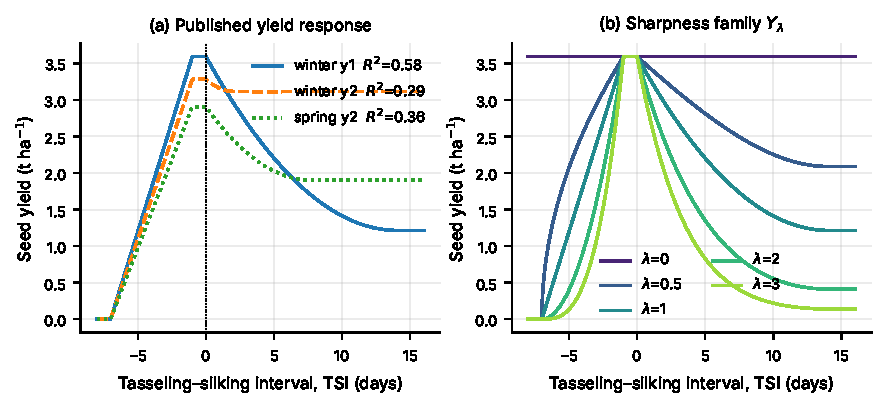
\includegraphics[width=\columnwidth]{../figs/fig1_yield_curve.pdf}
\caption{(a) Published yield--TSI regressions~\cite{marahatta2025}, with the
negative-TSI side supplied by the floral-overlap term. (b) The sharpness
family of \eqref{eq:sharp}; $\lambda = 1$ is the published response.}
\label{fig:curve}
\end{figure}

\subsection{Decision problem}

Let $x_{i,d,o} \in \{0,1\}$ indicate that field $i$ is sown with female day
$d$ and male offset $o \in \mathcal{O}$. Stage~1 solves
\begin{align}
\max \quad & \sum_{i \in \mathcal{F}} \sum_{d \in \mathcal{T}} \sum_{o \in \mathcal{O}}
  a_i \, \mathbb{E}_{\xi}\!\left[ Y_\lambda(\TSI_i(d,o,\xi)) \right] x_{i,d,o}
  \label{eq:obj}\\
\text{s.t.}\quad
& \sum_{d}\sum_{o} x_{i,d,o} \le 1, \qquad \forall i \in \mathcal{F}
  \label{eq:once}\\
& \sum_{i}\sum_{(d,o)\,:\, t \in V(d,o)} x_{i,d,o} \le K,
  \qquad \forall t \in \mathcal{T}
  \label{eq:cap}\\
& x_{i,d,o} = 0 \quad \text{if } V(d,o) \not\subseteq \mathcal{T},
  \label{eq:window}
\end{align}
where $\xi$ indexes weather scenarios and the expectation in
\eqref{eq:obj} is taken after each visit in $V(d,o)$ has slipped to the next
trafficable day in scenario $\xi$, so that rain-induced delay is priced
into the plan. Constraint~\eqref{eq:cap} is what couples the fields: it is
the reason a decision about one field changes the biology of another. A
field left unassigned contributes nothing; the solver leaves a field
unassigned only when \eqref{eq:cap} cannot accommodate it.

Stage~2 is a policy $\Psi$ mapping the information available on day $t$ to a
revised assignment for the fields not yet sown. Writing $\mathcal{I}_t$ for
that information set, we impose \emph{non-anticipativity}:
\begin{equation}
\Psi(t,\xi) = \Psi(t,\xi') \quad \text{whenever} \quad
\mathcal{I}_t(\xi) = \mathcal{I}_t(\xi').
\label{eq:nonantic}
\end{equation}
Two scenarios that are indistinguishable from what has been observed must
receive the same decision. Without~\eqref{eq:nonantic} a rolling-horizon
policy can quietly consult the future and any measured benefit is
meaningless.

% =========================================================================
\section{Strategies}
\label{sec:strategies}
% =========================================================================

We compare six policies. All share one execution engine, so differences
cannot come from differing accounting.

\begin{description}
\itemsep1pt
\item[\textbf{S1 Current practice.}] Each field receives the per-hybrid
offset that minimises its expected absolute TSI over the planning
ensemble at a reference date --- what a climatological degree-day table
encodes and what~\cite{chassaigne2021,asefa2024} advise. Fields are then
taken in a fixed order, each started on the first day the crew has
capacity. The agronomy is right; the logistics are naive.
\item[\textbf{S1$'$ Greedy dispatch.}] The same per-hybrid offsets and the
same expected-yield table that S3 uses, but assigned by a rule a supervisor
could follow or a short script could implement: fields are ordered
hardest-cross-first (largest absolute offset, then largest area), and each
takes the highest-expected-yield $(d,o)$ whose visit days still have crew
capacity. This is the ``could a simple script do it?'' competitor.
\item[\textbf{S2 Static (EV).}] Problem~\eqref{eq:obj}--\eqref{eq:window}
solved once against a single typical-season forecast.
\item[\textbf{S3 Static (robust).}] Solved once against a weather ensemble
with rain-induced slippage priced in. This is the plan a producer would
run from a tool that does not replan, and it is deliberately a
\emph{strong} baseline for S4.
\item[\textbf{S4 Dynamic.}] Starts from the S3 plan and re-optimises every
$q$ days on a conditional ensemble formed by historical analogue, described
below, subject to~\eqref{eq:nonantic}.
\item[\textbf{S5 Wait-and-see.}] Solved with perfect foreknowledge of the
realised season, with wet days excluded from the choice set. Not
implementable. It is a feasible perfect-information plan rather than
provably the best one, so the headroom it indicates is a lower bound on
the true value of perfect information.
\end{description}

The main result of the paper is S3 against S1 and S1$'$: the value of
solving the assignment. Following stochastic programming
convention~\cite{birge} we also report $\VSS = \text{S3} - \text{S2}$, the
value of modelling uncertainty at all; $\text{S4} - \text{S3}$, the value of
adaptivity; and $\EVPI = \text{S5} - \text{S4}$, the residual worth of
perfect information.

\subsection{Conditioning without inventing weather}

A rolling-horizon policy needs a conditional forecast: given the season so
far, what are the plausible remainders? The usual device is to splice the
observed prefix onto sampled climatological futures, and it is unavailable
here --- flowering comes from a crop model indexed by year, so a spliced
season is not one the model can run.

We therefore condition by \emph{historical analogue}. On each replanning day
the season to date is compared with the same calendar stretch of every other
year on record, scored on accumulated thermal time and cumulative rainfall,
and the closest $m$ years become the forecast ensemble. Early in the window
almost every year is a plausible analogue; as the season advances the set
narrows, and that narrowing \emph{is} the information the adaptive policy
has and the static plan does not. Non-anticipativity holds by construction:
similarity is computed only over elapsed days, and the realised season's
future is never read.

\subsection{Two details that decide the outcome}

Preliminary runs had the dynamic policy performing \emph{worse} than the
static one, for two reasons worth recording because both are easy to get
wrong. First, a rolling horizon free to reassign everything at each step can
defer a field indefinitely, each revision locally attractive, until the
window closes and the field is never sown; we freeze any operation within
$\ell$ days of its scheduled date, which is also operationally realistic.
Second, if the scenario-averaged objective already prices in rain slippage,
the optimiser must not \emph{also} forbid days that might be wet --- doing
both charges the same risk twice. We additionally adopt a revision only when
it improves the expected objective over the plan already in hand by more
than a tolerance $\epsilon$. Algorithm~\ref{alg:roll} gives the execution
loop shared by every strategy.

\begin{algorithm}[t]
\caption{Rolling-horizon execution (S4; S1--S3, S5 skip lines 3--8)}
\label{alg:roll}
\small
\begin{algorithmic}[1]
\STATE $P \leftarrow$ Stage-1 plan
\FOR{$t = 1$ \TO $T$}
  \IF{$t \bmod q = 0$ \AND $P \ne \emptyset$}
    \STATE build conditional ensemble from $\mathcal{I}_t$ \COMMENT{obeys \eqref{eq:nonantic}}
    \STATE freeze operations due within $\ell$ days
    \STATE $P' \leftarrow$ re-solve \eqref{eq:obj}--\eqref{eq:window} over unsown fields
    \STATE \textbf{if} $\mathrm{score}(P') > (1+\epsilon)\,\mathrm{score}(P)$ \textbf{then} $P \leftarrow P'$
  \ENDIF
  \STATE execute operations due by $t$, in planned order, while the field is
         trafficable and crew capacity remains; otherwise defer
\ENDFOR
\STATE \textbf{return} $\sum_i a_i Y_\lambda(\TSI_i)$ from realised sowing days
\end{algorithmic}
\end{algorithm}

\subsection{From model to tool}
\label{sec:tool}

As a decision-support tool the scheduler takes four inputs the producer
already holds or can download: (i) the field list with parent pair, area
and drainage class; (ii) the sowing window and crew capacity $K$; (iii) a
daily weather record for the site, from which the planning ensemble is
drawn; and (iv) a flowering model for each parent --- here a precomputed
CERES-Maize table, but a degree-day requirement from a seed catalogue
would serve. Its output is a calendar: for each field, the female sowing
day, the two male sowing days, and the expected yield; for each day, which
fields the crew visits. Fig.~\ref{fig:practice} shows one such calendar
beside the hand-made one it replaces. The plan is produced before the
season by a single exact solve (Section~\ref{sec:results} reports solve
times); if replanning is enabled, the same solve is repeated every $q$ days
on the fields not yet sown, using only weather observed to date. Nothing
in the pipeline requires a sensor on the field, and every component is
free software.

% =========================================================================
\section{Experimental Design}
\label{sec:design}
% =========================================================================

\subsection{Site and weather}

We study Ranebennur taluk, Haveri district, Karnataka
($14.60^\circ$N, $75.60^\circ$E, 597~m), which together with the adjacent
Ranebennur--Haveri belt is one of India's principal hybrid maize seed
production areas. Weather is twenty-one complete observed seasons,
2005--2025, from NASA POWER~\cite{power}: daily maximum and minimum
temperature, precipitation and solar radiation on the $0.5^\circ$ grid cell
containing the site. Nothing is generated. Every season a strategy is
evaluated on is a season that happened. Gridded reanalysis smooths local
rainfall relative to a station gauge, which if anything understates the
disruption the schedule must absorb.

Seed crops here are grown in the \emph{rabi} season, sown between
1~October and 30~November so that flowering falls in the dry December--January
window when pollen is not washed off the tassel. The sowing window is
therefore $T = 61$ days (day of year 274--334), and rain during it is the
disturbance the schedule must absorb. We take a field to be untrafficable
on any day with more than 5~mm of rain and for $\rho_i$ days afterwards,
where $\rho_i \in \{1,2,3\}$ is its drainage class. The threshold and the
recovery times are assumptions, not measurements; they stand in for the
soil-workability models of~\cite{bagheri2025}, and because every strategy
faces the same closures they affect the level of yield rather than the
comparison between strategies.

\subsection{Phenology}

Flowering dates come from CERES-Maize as implemented in
DSSAT-CSM~v4.8~\cite{dssat}, not from the degree-day approximation of
Section~\ref{sec:formulation}. For every combination of cultivar, season
and sowing day in the window we ran the model and recorded the simulated
anthesis date, giving a lookup table of $8 \times 21 \times 61 = 10{,}248$
entries; all of them reach anthesis. Simulations are run without water or
nitrogen limitation so that the table isolates the thermal and photoperiodic
control of flowering, which is the mechanism the scheduler reasons about.

The crop model, not the scheduler, supplies the reason adaptivity could
matter here: for a fixed pair of parents sown on a fixed date, the gap between
their flowering dates varies across the twenty-one seasons with a standard
deviation of 1.5~days on average over the parent pairs of a farm (median 1.4,
range 0.6--2.3). That variation is weather; it is unknown when the plan is
made; and at the measured penalty the first day of asynchrony costs 9.1\% of
seed yield.

\subsection{Farms}

The farms are synthetic instances on observed weather. The eight cultivars
are taken unmodified from DSSAT's distributed maize genotype file and span
50.2 to 66.3 days to anthesis at this site. Parent pairs are drawn from this
set so that the two lines of a field flower between 1.5 and 14 days apart,
which is the range over which staggered sowing is actually practised; pairs
are sampled across that range so that a farm contains both easy and
difficult crosses. Field areas are drawn uniformly from 1.5 to 4.0~ha and
drainage classes uniformly from $\{1,2,3\}$. Each configuration is
replicated across five independently drawn farms. Crew capacity is fixed at
$K = 2$ field-visits per day and farm size $N$ is swept from 10 to 70
fields, which moves \emph{resource pressure},
\[
  \pi \;=\; \frac{N \cdot V}{T \cdot K},
\]
the ratio of crew-visits demanded to crew-visits available ($V = 3$ visits
per field), from 0.25 to 1.72. At $\pi < 1$ the crew has slack; at $\pi > 1$
some fields cannot be served on their preferred days and the scheduling
problem binds.

\subsection{Protocol}

Evaluation is leave-one-season-out. Each scored season is held out, the
planning ensemble is eight seasons sampled with a fixed seed from the
remaining twenty, and no strategy ever sees the season it is tested on.
Every strategy is evaluated on the same held-out seasons, the same farms
and the same ensembles, so all comparisons are paired.

Two experiments differ in how many seasons they score, and we state the
difference because it matters. The \emph{assignment} experiment (S1, S1$'$,
S3, S5) needs one exact solve per strategy per season and is scored on all
twenty-one seasons. The \emph{replanning} experiment (S2--S5, with S4
re-solving every $q = 5$ days) is a dozen times more expensive and is
scored on seven of the twenty-one seasons --- every third year, 2005, 2008,
\dots, 2023, by a fixed rule rather than by selection. The replanning
experiment is also run on the sharpness sweep, at $\lambda \in \{0.25, 0.5,
1, 2, 3\}$ and fixed $\pi = 1.35$, and on a denser grid of farm sizes
around $\pi = 1$.

Gains are reported as the ratio of total extra seed to total baseline seed
over all farm--seasons in a cell, which is what a producer's accounts would
show and is the more conservative of the two available estimators;
intervals are bootstraps that resample whole farms, since seasons within a
farm are not independent. Where we report $p$-values they are from paired
$t$-tests on farm--season differences and should be read as descriptive,
given the number of cells.

Stage-1 and each replan are solved with CBC~\cite{cbc}
through PuLP. Every one of the 1155 stage-1 problems in the assignment experiment was solved to proven optimality, in at most 58~s (Table~\ref{tab:solver}). Re-solves inside the replanning loop run under a 12-second limit; a re-solve that reaches it returns its incumbent, which is then subject to the adoption test, so a time-limited revision can only be adopted if it is already better than the plan in hand. As a check on the machinery we reran the
dynamic strategy with its adoption threshold set so high that no revision
is ever accepted; it reproduced S3 exactly, confirming that the measured
gain from replanning comes from adopted revisions and not from an
implementation difference between the two arms.

% ---------------------------------------------------------------------------
\section{External Validation}
\label{sec:validation}

A simulation is only as good as the biology inside it, so we test the model
against a dataset that played no part in building it.
Chassaigne-Ricciulli \textit{et al.}~\cite{chassaigne2021} report, for six
three-way-cross tropical maize hybrids at CIMMYT's station in Agua Fr\'ia,
Mexico, the parents' accumulated degree days at flowering, the differential
sowing interval they recommend, and a ranking of the six by difficulty of
seed production. None of it entered our model: the yield response comes from
Nepal~\cite{marahatta2025} and the phenology from DSSAT~\cite{dssat}.

Three of our parameters are corroborated. Both studies compute thermal time
identically, above a $10^\circ$C base and truncated at $30^\circ$C. CIMMYT
estimate ``7 days for the total pollen shedding duration,'' the value our
floral-overlap term assumes, and report stigmas receptive about five days
after the onset of female flowering, inside our six-day window --- so the one
component we extended beyond the fitted data is supported by measurements
from another continent. The model's core claim, that the offset needed to
synchronise two parents equals their thermal-time difference divided by the
rate of degree-day accumulation, predicts their recommended offsets with a
mean absolute error of 1.5~days and recovers the correct direction in six
cases of six (Fig.~\ref{fig:cimmyt}(a)); ranking the same hybrids by the
offset our model requires reproduces their own difficulty ordering at
Spearman $\rho = 0.71$ (Fig.~\ref{fig:cimmyt}(b)), suggestive rather than
significant at $n = 6$.

Two caveats bound what this buys. The test exercises the thermal-time rule
of Section~\ref{sec:formulation}, which is the mechanism CERES-Maize
implements with additional photoperiod and leaf-appearance terms; it does
not exercise CERES-Maize's cultivar coefficients, which are DSSAT's and not
CIMMYT's. And the 1.5-day error is of the same order as the 1.5-day
season-to-season variation in the flowering gap that in-season replanning
exploits, so the validation supports the main result --- the value of
solving the assignment, which turns on the mean offsets and on crew
throughput --- more strongly than it supports the finer replanning result.
It does not validate the scheduler: no one has executed one of our
schedules on real fields and weighed the resulting seed. What it buys is
the right to read differences between strategies as differences in
scheduling quality rather than artefacts of a misspecified crop response.

\begin{figure}[t]
\centering
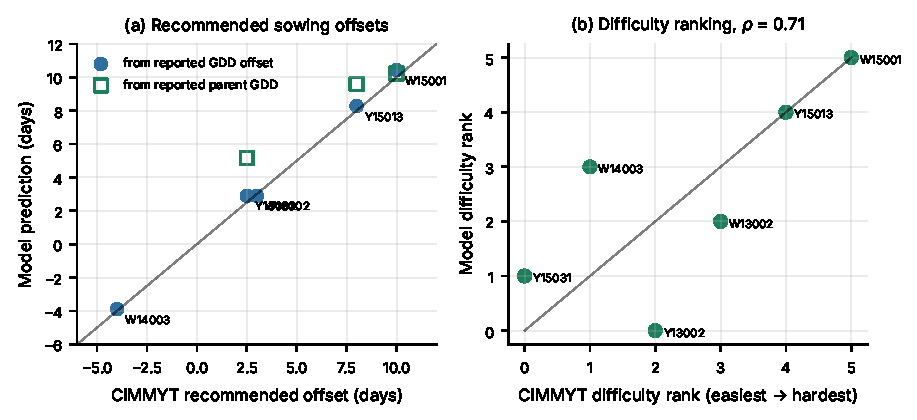
\includegraphics[width=\columnwidth]{../figs/fig7_cimmyt.pdf}
\caption{External validation against CIMMYT's published seed-production
recommendations~\cite{chassaigne2021}. (a) Predicted against recommended
sowing offsets for six three-way-cross hybrids; the line is parity.
(b) Hybrid difficulty ranking.}
\label{fig:cimmyt}
\end{figure}

% =========================================================================
\section{Results}
\label{sec:results}
% =========================================================================

\subsection{The optimised assignment against current practice}

Table~\ref{tab:solution} gives the main result on all twenty-one
seasons. Against current practice (S1) the optimised assignment (S3)
yields $+11.9$\% more seed pooled over every farm size
(95\% farm-bootstrap CI $+11.0$ to $+12.7$\%),
rising to $+38$\% at $N = 70$ fields. The gain is
193~kg of hybrid seed per hectare per season on average and
448~kg\,ha$^{-1}$ at $N = 70$, with no change to
inputs, genetics or acreage, and it is sold at hybrid-seed rather
than grain prices.

The mechanism is visible in Fig.~\ref{fig:practice} and in the
fields-sown columns of the table. Working through fields in order and
taking the first free slot fills the calendar from the front and runs
out of window: current practice places about 39 fields
however many it is given, so at $N = 70$ it sows
39 and abandons the rest, while the
optimised plan places 59. The
same crew, the same window and the same weather serve half again as
many fields.

Where the extra throughput comes from is worth stating exactly,
because it is the model's central assumption. With $K = 2$ visits a day
over 61 days the crew has 122 visits; at three visits per field that
is about 40 fields, which is where current practice saturates. The
optimiser gets past 40 by choosing, for some fields, an offset at which
one of the male sowings falls on the female's day ($o = 0$ or
$o = -\delta$), so the field needs two visits instead of three ---
Section~\ref{sec:formulation}, Eq.~\eqref{eq:visits}. Those offsets
are not the synchrony-optimal ones for most parent pairs, which is
why the optimised plan's mean asynchrony is larger. The gain is
therefore a trade the supervisor could in principle make by hand but
does not, because deciding \emph{which} fields should give up a day
of synchrony to free a crew-day for \emph{which other} field is
exactly the coupled decision that is hard to make by hand. Whether
the trade is available at all depends on capacity being limited by
visits to isolated fields rather than by rows sown; we test the
alternative below.

The gain is not free and we report the price. The optimiser accepts
slightly worse synchrony on each field --- mean absolute TSI
5.4 days against
4.1 for current practice at
$N = 70$ (Fig.~\ref{fig:practice}(c)) --- in exchange for
serving far more of them. That trade is the whole content of the
decision: a scheduler that insisted on perfect synchrony everywhere
would sow fewer fields and produce less seed in total. Below
saturation, where every field can be served, the gain comes instead
from choosing \emph{which} day each field gets, and is smaller.

\subsection{Is an exact solver needed?}

The greedy dispatcher S1$'$ is given the same per-hybrid offsets and
the same ensemble expected-yield table as the optimiser, and differs
from it only in assigning fields one at a time, hardest first, rather
than jointly. Pooled over all configurations the exact solution
yields $+12.4$\% more than the greedy
(95\% CI $+11.2$ to $+13.7$\%);
$+0.6$\% where the crew has slack ($\pi < 0.9$),
$+6.2$\% near saturation and $+25.0$\% under
over-subscription ($\pi > 1.1$).
The two regimes tell different stories. Where the crew has slack
the greedy is as good as the exact solver: the fields do not compete
for days, so assigning them one at a time loses nothing, and the
$+6.1$\% it gains over current practice there is the
value of \emph{what the dispatcher knows} --- an expected-yield
table built from a crop model and a weather ensemble --- rather than
of how it searches. Under over-subscription the greedy collapses:
it does $-3.6$\% relative to current practice, i.e.
worse, because taking the best slot for each hard field in turn
spends the contested crew-days on synchrony and leaves later fields
with nowhere to go (it sows 37 of
70 fields against practice's 39
and the optimiser's 59). The
trade that produces the headline gain --- giving up a day of
synchrony on some fields to free crew-days for others --- is a
joint decision, and a one-field-at-a-time rule cannot make it
however it is ordered. A sensible script is therefore not enough
at exactly the scale where the problem matters, and since the exact
solve costs seconds (Table~\ref{tab:solver}) there is no reason to
settle for one.

\begin{table}[t]
\centering
\caption{Optimised assignment against current practice, all 21 seasons}
\label{tab:solution}
\setlength{\tabcolsep}{3.5pt}\footnotesize
\begin{tabular}{rrrrrrrrr}
\hline
 & & \multicolumn{3}{c}{mean yield (t)} & \multicolumn{2}{c}{fields sown} & \multicolumn{2}{c}{S3 gain over} \\
$N$ & $\pi$ & S1 & S1$'$ & S3 & S1 & S3 & S1 & S1$'$ \\
\hline
10 & 0.25 & 56 & 66 & 65 & 10 & 10 & $+16.5$\% & $-0.5$\% \\
20 & 0.49 & 114 & 127 & 127 & 20 & 20 & $+11.3$\% & $-0.3$\% \\
30 & 0.74 & 167 & 178 & 180 & 30 & 30 & $+7.6$\% & $+1.0$\% \\
35 & 0.86 & 207 & 206 & 209 & 35 & 35 & $+0.8$\% & $+1.1$\% \\
37 & 0.91 & 212 & 212 & 215 & 37 & 37 & $+1.3$\% & $+1.7$\% \\
40 & 0.98 & 228 & 222 & 235 & 39 & 39 & $+3.0$\% & $+5.9$\% \\
43 & 1.06 & 224 & 220 & 244 & 39 & 42 & $+8.6$\% & $+10.9$\% \\
45 & 1.11 & 222 & 216 & 249 & 39 & 44 & $+12.1$\% & $+15.2$\% \\
48 & 1.18 & 224 & 218 & 254 & 39 & 47 & $+13.1$\% & $+16.5$\% \\
55 & 1.35 & 223 & 214 & 266 & 39 & 54 & $+18.9$\% & $+24.3$\% \\
70 & 1.72 & 229 & 219 & 315 & 39 & 59 & $+37.8$\% & $+43.9$\% \\
\hline
\end{tabular}
\\[2pt]
\footnotesize\raggedright Each row is 5 independently drawn farms
$\times$ 21 held-out seasons ($n = 105$). Gains are ratios of unrounded
totals within the row. S1: current practice; S1$'$: greedy dispatch; S3:
optimised assignment.
\end{table}

\begin{figure*}[t]
\centering
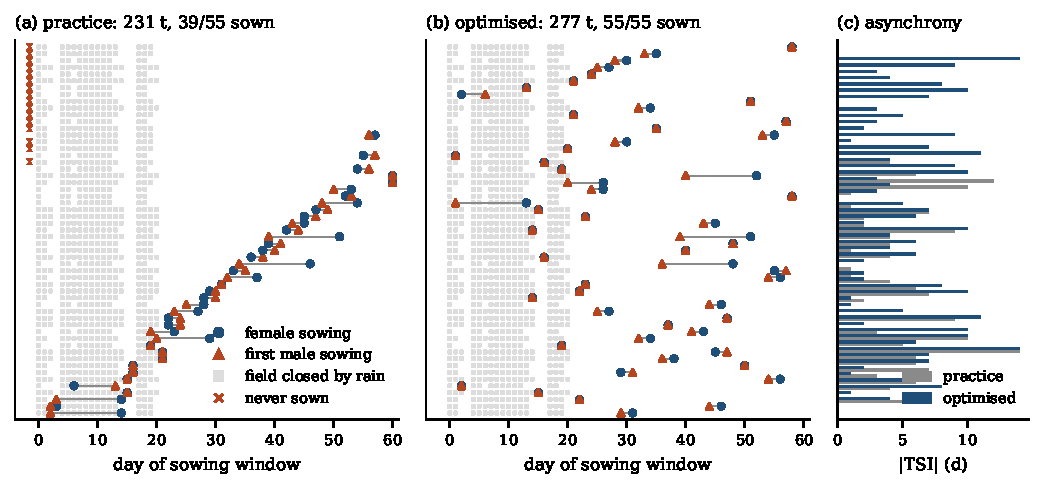
\includegraphics[width=\textwidth]{../figs/fig12_practice.pdf}
\caption{What the tool changes. One farm ($N = 55$, $K = 2$,
$\pi = 1.35$) in the 2022 season, chosen as the season whose gain is
closest to the median over all twenty-one. (a) Current practice fills
the calendar from the front with the recommended offsets and runs out
of window; sixteen fields are never sown. (b) The optimised assignment
spreads the fields across the window and sows all of them. (c) The
price: realised asynchrony per field is slightly larger under the
optimised plan, which it accepts in exchange for serving every field.}
\label{fig:practice}
\end{figure*}

\subsection{Solve time}

Table~\ref{tab:solver} gives the size of the stage-1 problem and CBC
wall time on one CPU core. The problem is small by
the standards of mixed-integer programming
(57890 binaries at $N = 70$), and
every instance solved to proven optimality. A producer
would run the stage-1 solve once before the season and each replan
in under a minute.

\begin{table}[t]
\centering
\caption{Stage-1 problem size and solve time}
\label{tab:solver}
\footnotesize
\begin{tabular}{rrrr}
\hline
$N$ & binaries & mean (s) & max (s) \\
\hline
10 & 8270 & 0.5 & 0.8 \\
20 & 16540 & 1.1 & 1.8 \\
30 & 24810 & 2.2 & 4.5 \\
40 & 33080 & 8.2 & 42.8 \\
55 & 45485 & 6.4 & 20.2 \\
70 & 57890 & 4.3 & 8.8 \\
\hline
\end{tabular}
\\[2pt]
\footnotesize\raggedright 1155 solves; status optimal in all cases.
\end{table}

\subsection{Sensitivity to the yield response}

The primary analysis scores synchrony with the best-fitting of the
three usable regressions in~\cite{marahatta2025}. Table~\ref{tab:curves}
repeats the assignment experiment with each alternative fit as both
objective and scorer, on all twenty-one seasons at three farm sizes.

\begin{table}[t]
\centering
\caption{Gain of S3 over S1 under each published yield response}
\label{tab:curves}
\footnotesize
\setlength{\tabcolsep}{3pt}
\begin{tabular}{@{}lrrrr@{}}
\hline
response & $N=10$ & $N=40$ & $N=70$ & pooled \\
\hline
winter y1, $R^2=0.58$ (primary) & $+17$\% & $+3$\% & $+38$\% & $+20.0$\% \\
winter y2, $R^2=0.29$ & $+6$\% & $+2$\% & $+69$\% & $+32.0$\% \\
spring y2, $R^2=0.36$ & $+13$\% & $+2$\% & $+51$\% & $+24.7$\% \\
\hline
\end{tabular}
\end{table}

The pooled gain ranges from $+20.0$\% to $+32.0$\%
across the three fits, and the primary curve gives the
smallest figure. Under the flatter fits the gain at scale is larger,
not smaller ($+38$\%, $+69$\%, $+51$\%
at $N = 70$): when a day of asynchrony costs less, the
visit-merging trade of Section~\ref{sec:results}-A is cheaper and the
optimiser makes it more often. The result does not depend on having
chosen the steepest curve; the primary curve is the conservative
choice.

\subsection{Sensitivity to the visit accounting}

If the crew's limit were sowing operations rather than visits to
fields, the merged-visit offsets would save nothing. We re-ran the
assignment experiment with $o = 0$ and $o = -\delta$ removed from
the choice set of every strategy, so that every field needs three
distinct crew days (Table~\ref{tab:nomerge}).

\begin{table}[t]
\centering
\caption{Gain of S3 over S1 with visit merging disallowed}
\label{tab:nomerge}
\footnotesize
\begin{tabular}{lrrrr}
\hline
 & $N=40$ & pooled \\
\hline
merging allowed (Table~\ref{tab:solution}) & $+3$\% & $+3.0$\% \\
merging disallowed & $+3$\% & $+3.3$\% \\
fields sown, S1 / S3 & 39 / 40 & \\
\hline
\end{tabular}
\end{table}

The gain falls to $+3.3$\% but does not vanish: with
every field costing three days, the crew can serve about 40
fields whatever the plan, and the optimiser's remaining advantage
is in choosing which fields to serve --- larger ones, and those
whose parents are easiest to synchronise in the days available ---
and when. A producer whose crew is limited by rows sown rather than
by field visits should expect the smaller figure.

\subsection{Where the remaining value lies}

The remaining results are from the replanning experiment (seven held-out
seasons). At the tightest configuration --- $N = 70$,
$K = 2$, $\pi = 1.72$ --- mean realised
seed yield rises along the ladder:
S1 current practice 230.8~t, S2 optimised, single forecast 300.4~t, S3 optimised, robust 310.1~t, S4 optimised, replanned 325.2~t, S5 wait-and-see bound 383.1~t.
Three quantities here are the ones stochastic programming
names~\cite{birge}. The value of the stochastic solution, S3$-$S2, is
9.7~t (3.2\%): planning against an
ensemble of seasons rather than one typical season is worth having,
though it is second-order next to solving the assignment at all. The
value of adaptivity, S4$-$S3, is 15.2~t. The expected value of
perfect information, S5$-$S4, is at least 57.8~t
(17.8\%; a lower bound, since S5 is a feasible
rather than provably optimal perfect-information plan): headroom a
perfect seasonal forecast would buy and no causal strategy can reach.
The ordering
S1 $<$ S2 $<$ S3 $<$ S5 is what theory requires and we use it as a
check on the implementation; theory does \emph{not} fix where S4
falls relative to S3, since a revision is adopted on a forecast that
may be wrong.

\subsection{Should the tool replan? Resource pressure}

Table~\ref{tab:pressure} and Fig.~\ref{fig:pressure} give the gain
from in-season replanning, S4 over S3, across resource pressure.
Pooled over every configuration it is
$+2.26$\% of realised seed yield (95\% farm-bootstrap
CI $+1.74$ to $+2.86$\%, $n = 315$
farm--seasons, Cohen's $d = 0.29$), positive on
38 of the 45 farm--configuration combinations.
The effect is small by conventional standards, which is the honest
description of an addition that costs nothing to apply once the
optimiser exists.

\begin{table}[t]
\centering
\caption{Value of in-season replanning against resource pressure}
\label{tab:pressure}
\footnotesize
\begin{tabular}{rrrrrr}
\hline
$N$ & $\pi$ & S3 (t) & S4$-$S3 & $p$ & $n$ \\
\hline
10 & 0.25 & 65.2 & $+7.25$\% & 0.018 & 35 \\
20 & 0.49 & 127.5 & $+4.00$\% & 0.022 & 35 \\
30 & 0.74 & 184.4 & $+1.37$\% & 0.392 & 35 \\
35 & 0.86 & 203.3 & $+1.62$\% & 0.378 & 21 \\
37 & 0.91 & 217.1 & $+1.29$\% & 0.546 & 21 \\
40 & 0.98 & 236.3 & $-2.53$\% & 0.060 & 35 \\
43 & 1.06 & 237.2 & $+1.90$\% & 0.488 & 21 \\
45 & 1.11 & 243.9 & $+0.74$\% & 0.677 & 21 \\
48 & 1.18 & 246.7 & $+2.69$\% & 0.099 & 21 \\
55 & 1.35 & 260.0 & $+3.61$\% & 0.009 & 35 \\
70 & 1.72 & 310.1 & $+4.90$\% & 0.000 & 35 \\
\hline
\end{tabular}
\\[2pt]
\footnotesize\raggedright Each row is 3 or 5 independently drawn farms
$\times$ 7 held-out seasons; $p$ from paired $t$-tests, descriptive.
\end{table}

We expected the gain to grow with resource pressure, on the reasoning
that an idle crew leaves a revision nothing to reallocate. It does not.
It is $+7.25$\% where the crew has the most
slack ($\pi = 0.25$), falls to
$-2.53$\% at $\pi = 0.98$ where capacity almost
exactly equals demand, and recovers to $+4.90$\%
($p < 10^{-4}$) at $\pi = 1.72$.
Pooling every farm--season with
$0.9 \le \pi \le 1.1$ gives
$+0.56$\% ($n = 77$) against
$+4.25$\% outside it ($n = 238$;
$p = 0.013$, Welch). The band is not
distinguishable from zero ($p = 0.654$), so the
defensible statement is that the gain \emph{vanishes} near
saturation, not that it reverses.

Three regimes explain this. With \emph{slack} a revision can be
executed and is mostly used to recover a field that rain pushed off
its planned day, so the benefit is insurance-shaped --- at
$\pi = 0.25$ only
57\% of
farm--seasons improve, the mean carried by rare seasons in which a
field the static plan loses is rescued. At \emph{saturation} every
revision is a forced swap whose achievable gain is small while the
forecast error motivating it is not, and the benefit washes out.
Under \emph{over-subscription} not every field can be served whatever
is done, so the decision becomes which to serve and which to concede
--- robust to forecast error in a way fine timing adjustments are not
--- and the gain returns.

\subsection{Should the tool replan? Penalty sharpness}

Fig.~\ref{fig:sharpreal} sweeps $\lambda$ at fixed $\pi = 1.35$.
Every member of the family shares the same optimum and maximum;
$\lambda$ changes only how fast yield falls away from it.
The gain rises monotonically with sharpness ($r = 0.96$, $p = 0.008$),
from $+0.49$\% at $\lambda = 0.25$
(95\% CI $-0.83$ to $+1.81$\%, a null
rather than merely a non-significant result)
to $+9.14$\%
(95\% CI $+5.07$ to $+13.77$\%)
at $\lambda = 3$. The flat end is the irrigation
regime, and we reproduce the irrigation result there: when the
biological penalty is nearly flat, re-optimising during the season
against a strong robust static plan buys essentially nothing, on the
same farms, weather and solver that deliver a significant gain when
the penalty is sharp. The difference between the two conclusions is
the response surface, not the method.
Five percent is the figure at which the irrigation literature judged
in-season adaptation not worth the cost of building it; interpolating
between sweep points, the gain passes it at $\lambda \approx 1.3$,
a penalty about half again as sharp as the one measured for hybrid
maize seed. Hybrid seed production therefore sits close to the
threshold, which is why it was worth measuring rather than assuming.

Sharpness and resource pressure act differently: the gain is monotone
in the first and not in the second, because sharpness sets how much a
timing error costs while pressure sets whether anything can be done
about it. An earlier sweep of $\lambda$ run at the saturated
configuration found no relationship at all --- a property of the
operating point, not of the biology.


\begin{figure}[t]
\centering
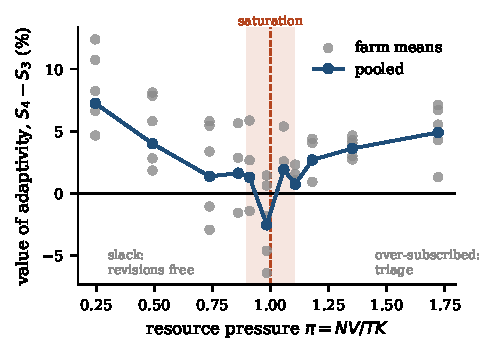
\includegraphics[width=\columnwidth]{../figs/fig8_pressure.pdf}
\caption{Value of in-season replanning against resource pressure, on seven
held-out seasons at Ranebennur. Grey points are individual farm means; the
line is pooled over the farms. The shaded band marks saturation, where the
crew's capacity equals the visits demanded.}
\label{fig:pressure}
\end{figure}

\begin{figure}[t]
\centering
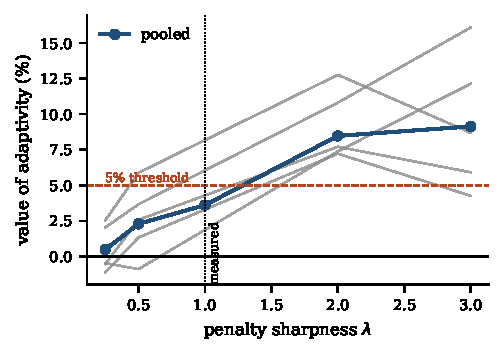
\includegraphics[width=\columnwidth]{../figs/fig9_sharpness_real.pdf}
\caption{Value of in-season replanning against penalty sharpness at
$\pi = 1.35$, where the crew binds. Grey lines are the five individual
farms. $\lambda = 1$ is the response published for hybrid maize seed;
$\lambda \to 0$ is the flat regime in which the irrigation literature found
adaptation not worth its cost.}
\label{fig:sharpreal}
\end{figure}


% =========================================================================
\section{Does field-level soil-temperature sensing change the schedule?}
\label{sec:iot}

\subsection{The gap the sensor would fill}

CERES-Maize does not run the phase that sets flowering date on air
temperature. While \texttt{LEAFNO .LE. 10}, \texttt{MZ\_PHENOL.for} (lines
457--496) forms daily thermal time from \emph{soil} temperature, estimated
from air temperature and solar radiation:
\begin{align}
a &= 0.01061\,\mathrm{SRAD} + 0.5902, \label{eq:acoef}\\
T_{\mathrm{day}} &= a\,T_{\max} + (1-a)\,T_{\min}, \label{eq:tdsoil}\\
T_{\mathrm{night}} &= 0.36354\,T_{\max} + 0.63646\,T_{\min}, \label{eq:tnsoil}\\
\Delta T\!T &= \tfrac{1}{2}\!\left[\max(T_{\mathrm{night}},T_b)
  + \min(T_{\mathrm{day}},D_{\mathrm{opt}})\right] - T_b, \label{eq:dtt}
\end{align}
with $T_b=8.0$ and $D_{\mathrm{opt}}=34.0$\,\textdegree C from the shipped
ecotype file, $\Delta TT$ then capped at $D_{\mathrm{opt}}-T_b$. The clamps
in~\eqref{eq:dtt} apply to each component \emph{before} the average: a
$40/20$\,\textdegree C pair yields $19.0$, averaging first $22.0$.
Crucially, \eqref{eq:acoef}--\eqref{eq:tnsoil} contain no field-specific
term, so two fields under one weather station receive identical estimated
soil temperature whatever their soil does. That imputation is the gap a
buried probe would close, and the only point where a soil-temperature
measurement has anywhere to enter.

\subsection{Simulation design}

\textbf{Nothing here is a measurement.} No soil-temperature observation was
obtained for this study. Paired 5\,cm bare and vegetated probes exist in the
Oklahoma Mesonet but sit behind an interactive request form and a
robots-disallowed endpoint; USCRN publishes no probe-level soil temperature,
its readme files stating the reported values are ``calculated from these
multiple independent measurements''. The sensing layer is explicitly
simulated and every parameter of it is recorded on each result row.

We implement \eqref{eq:acoef}--\eqref{eq:dtt} directly and calibrate one
thermal threshold per cultivar against the existing DSSAT table ($n=1281$
per cultivar), reproducing it to $2.62$\,d RMSE with mean absolute bias
$0.14$\,d against $2.70$\,d for the same arithmetic on air temperature.
This is a self-consistent substrate, not a claim to reproduce DSSAT: truth
and all planners run on it, so its absolute error cancels in the paired
comparison and its bias --- which would not --- is near zero.

Each field receives a constant soil thermal offset $\delta_i$. The default
scale $\sigma=0.7$\,\textdegree C is \emph{not} chosen here: it is the value
already carried by \texttt{sim.core.make\_farm}, committed before this
analysis existed. $\sigma$ is swept from $0$ regardless, and $\sigma=0$ is a
null scenario in which a sensor must show no gain. A virtual probe reads the
field's soil temperature with Gaussian noise of $0.5$\,\textdegree C --- the
documented accuracy of the Mesonet thermistors whose data we could not
obtain --- and misses days at a configurable rate; $\hat\delta_i$ is the
mean over observed days of the residual against what
\eqref{eq:tdsoil}--\eqref{eq:tnsoil} would impute. Observation closes on day
273, before the window opens on day 274, so the channel is
non-anticipative: a field offset is a persistent property, not a forecast.

Three planners differ only in belief: \textsc{conventional} believes every
offset is zero, exactly what CERES does; \textsc{sensor} believes
$\hat\delta_i$, falling back to zero where estimation failed;
\textsc{oracle} believes the truth and bounds the gain. Everything else ---
fields, parent pairs, areas, weather years, capacity model and budget,
response scenario, objective, candidate enumeration --- is the same object
for all three, and every coefficient and executed score passes through one
scoring function.

\subsection{Capacity must bind before the question is meaningful}

At the farm size used elsewhere here the capacity constraint is almost
inactive --- at $N=12$ the constrained optimum is within $0.06\%$ of the
unconstrained one --- so measuring the value of information there measures
nothing about scarcity. At $N=60$ it binds properly, $17.7\%$ of objective
under the visits model, with only $53$ of $60$ fields sown. All
capacity-constrained results use $N=60$.

\subsection{Results}

\begin{table}[t]
\centering
\caption{Change in objective against the conventional CERES pathway.
Capacity-constrained rows: visits model, $N=60$, 6 farm seeds per level
($\sigma=0.7$ repeated at 12 seeds gives $+0.583\%$ $[+0.435,+0.732]$).
95\% confidence intervals across seeds.}
\label{tab:iot}
\begin{tabular}{lrrrrr}
\toprule
$\sigma$ (\textdegree C) & sensor (\%) & 95\% CI & seeds $>0$ & oracle (\%) & captured \\
\midrule
\multicolumn{6}{l}{\emph{capacity-constrained, $N=60$}}\\
0.00 & $-1.410$ & $[-1.505,-1.316]$ & 0/6 & $+0.000$ & --- \\
0.50 & $+0.455$ & $[+0.296,+0.615]$ & 6/6 & $+2.005$ & 0.23 \\
0.70 & $+0.563$ & $[+0.392,+0.735]$ & 6/6 & $+2.279$ & 0.25 \\
1.00 & $+1.050$ & $[+0.836,+1.263]$ & 6/6 & $+2.792$ & 0.38 \\
2.00 & $+2.125$ & $[+1.789,+2.462]$ & 6/6 & $+3.891$ & 0.55 \\
4.00 & $+6.065$ & $[+2.972,+9.157]$ & 6/6 & $+7.493$ & 0.81 \\
\bottomrule
\end{tabular}
\end{table}

\textbf{Scarcity makes the information worth having.} Matched at $N=60$ and
$\sigma=0.7$, the sensor gains $+0.191\%$ $[-0.008,+0.389]$ without a
binding capacity constraint --- an interval spanning zero --- and
$+0.583\%$ $[+0.435,+0.732]$ with one, positive in all twelve seeds; the
oracle rises from $+1.642\%$ to $+2.279\%$ over the same contrast.
Information about which fields run warm is worth more when the crew cannot
serve every field, because it then also informs \emph{which} fields to sow.

\textbf{Scarcity also makes noise more expensive.} At $\sigma=0$ the oracle
gain is exactly zero, as it must be, while the sensor loses $1.410\%$
$[-1.505,-1.316]$, negative in every seed, against $0.164\%$ unconstrained.
Noise read as real offset does not merely mis-set an offset; under scarcity
it misallocates a day the crew cannot get back.

\textbf{A realistic probe leaves three quarters of the value unclaimed.} A
noise ablation at $\sigma = 0.7$, six seeds, isolates why: a noiseless probe
recovers the oracle \emph{exactly} ($+2.279\%$ against $+2.279\%$), and the
captured share falls to $0.41$ at $0.25$\,\textdegree C, $0.25$ at
$0.5$\,\textdegree C, $0.20$ at $1.0$ and $0.15$ at $2.0$. The limiting
quantity is instrument accuracy, not the scheduler and not the observation
campaign. Estimation degrades gracefully by comparison: losing three
quarters of the observations moves the captured share only from $0.25$ to
$0.18$, and with every observation lost the gain is exactly $+0.000\%$ with
no plan changed, confirming the zero-belief fallback.



\textbf{Solver validity.} Every capacity-constrained cell above was solved
on the visits model with measured LP gap median $0.0001$, maximum $0.0003$,
inside the $0.005$ acceptance rule, and no arm hit the time limit. The
operations, hours and hectares models do not reach that standard at $N=60$
and more solver time does not help: at a 45\,s limit every arm terminated
time-limited with gaps $0.011$--$0.034$, and raising the limit to $300$\,s
left the gaps on the same cell unchanged to five decimals
($0.01140$, $0.02253$, $0.01441$) at twenty times the cost. The limitation
is LP bound quality for these cost structures, not search time. Those cells
are lower bounds, their spread exceeds the effect measured, and one produced
a negative oracle gain that cannot be real, so they are excluded from
inference. Robustness to capacity accounting is therefore \emph{not}
established here.

\subsection{What this does and does not establish}

It establishes, inside this model and with simulated sensing, that the
decision value of per-field soil-temperature measurement is governed by the
ratio of between-field heterogeneity to probe accuracy and by how tightly
sowing capacity binds. Both raise the gain, and scarcity raises the cost of
error at the same time. That is a transferable criterion for when such a
system is worth building.

It does not establish what the between-field heterogeneity of a commercial
seed-production block actually is. Published same-site contrasts at 5\,cm
run 1--6\,\textdegree C between deliberately imposed treatments, but such a
block is managed uniformly, and the one continuous relationship available
--- soil temperature against percent residue cover --- implies
$0.11$--$0.59$\,\textdegree C between fields under one protocol. At the top
of that range the constrained sensor gains about $+0.46\%$; at the bottom it
is indistinguishable from zero and, if the fields are truly identical,
actively harmful. Establishing the real figure requires paired measurements
we were unable to obtain. The emulator's 2.6\,d RMSE against DSSAT also
exceeds the one-day decision unit; the paired comparison cancels this, but
it would not cancel for any absolute claim about flowering date. \textbf{No seed-yield
improvement is claimed and no physical sensor was deployed or tested}: the
objective is this study's own area-weighted relative-yield response to the
anthesis--silking interval.


\begin{figure*}[t]
\centering
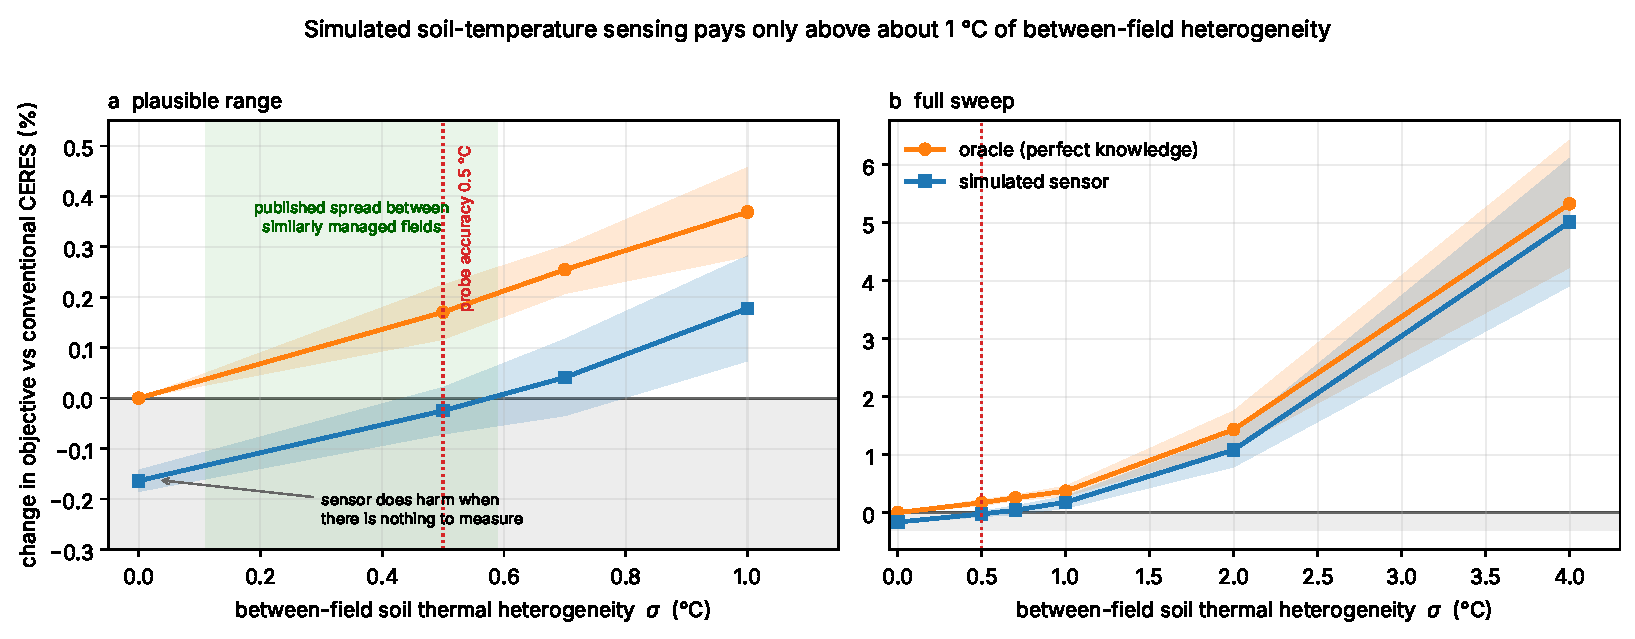
\includegraphics[width=\textwidth]{../figs/fig13_iot_decision_value.pdf}
\caption{Decision value of simulated per-field soil-temperature sensing.
(a) Between-field heterogeneity, capacity-constrained ($N=60$) against
unconstrained ($N=12$); the red diamond is the matched unconstrained case at
$N=60$ and $\sigma=0.7$, and the green band is the spread published for
similarly managed fields. (b) Probe noise; percentages are the share of the
oracle gain captured. (c) Missing observations. Bands are 95\% confidence
intervals across farm seeds. All sensing is simulated.}
\label{fig:iot}
\end{figure*}

\section{Discussion}
% =========================================================================

\subsection{What to build, and in what order}

The results separate into something every producer at scale should do
and something only some should.

\emph{Solve the assignment before the season.} This is worth
$+11.9$\% overall and $+38$\% at scale, needs no
forecast, no in-season data collection and no change to agronomy, and
the whole stack is free software running in seconds. Its benefit grows
with farm size because the constraint it removes --- naive sequencing
saturating near 39 fields --- bites harder the more
contracts a producer carries. Below saturation the gain is modest and
a producer with a small contract book may reasonably not bother.

\emph{Add replanning only under two conditions.} The penalty must be
sharp: where a day of timing error costs little, a robust static plan
absorbs the risk in advance, which is what the irrigation studies
found and what we reproduce at $\lambda = 0.25$
($+0.49$\%, $p = 0.444$). And the schedule must have
room to move: a revision is only worth making where a field can go
somewhere, which is why the gain vanishes at saturation and returns on
either side. Both conditions are arithmetic --- a published response
curve and $\pi = NV/TK$ --- so a producer can decide before any
software is written. An operation that has sized its crew precisely
to its acreage should optimise its schedule and leave it alone.

\subsection{Scope of the irrigation result, and what remains}

Kelly \textit{et al.}~\cite{kelly2023} and Becker \textit{et
al.}~\cite{becker2026} are right about irrigation, and we reproduce
their finding at the flat end of our sharpness family. Our claim is
narrower than a contradiction: their conclusion describes a region of
a two-dimensional space --- how sharply the biology punishes a timing
error, and how much freedom the operation has to correct one ---
rather than agricultural scheduling as such. Irrigation sits at the
null end of both.

Finally, the oracle beats the best causal strategy by at least 57.8~t
at the tightest configuration, several times the value of replanning
itself. Most of what a perfect seasonal forecast would buy is
unclaimable by better optimisation alone: the non-anticipativity
constraint, not the solver, stands in the way. The route to it is
forecast skill at the four-to-eight-week range over the flowering
window.


% =========================================================================
\section{Limitations}
\label{sec:limits}
% =========================================================================

\emph{This is a simulation study.} No seed was produced. The results say
when these schedules are worth \emph{testing} in the field, not that a given
gain will be realised on a given farm.

\emph{Current practice is described from the literature, not observed.}
We have not interviewed a producer or obtained a hand-made schedule. The
baseline encodes what the agronomic recommendations say to do per field and
the operational assumption those recommendations state~\cite{chassaigne2021};
a producer who already sequences fields by difficulty would be closer to
S1$'$ than to S1, and we report both.

\emph{The farms are synthetic.} The weather, the site and the crop model are
real; field areas, drainage classes, parent pairs and crew capacity are
sampled or assumed. The parents are public DSSAT cultivars, not the
proprietary inbreds of any commercial hybrid. A producer's own calibration
would shift the required offsets without changing the structure of the
result, which depends on how variable the parent flowering gap is across
seasons and on how hard the crew is worked rather than on the gap's mean.
Flowering is simulated without water or nitrogen limitation; under stress
asynchrony would be larger and more weather-dependent, which would if
anything raise the value of both optimising and replanning.

\emph{The yield response is from one site and extended on one side.} The
regression is from Chitwan, Nepal, applied at a Karnataka site; it is the
only published quantitative seed-yield-versus-TSI response we could find.
Section~\ref{sec:validation} tests its parameters elsewhere rather than
assuming they transfer, and Section~\ref{sec:results} repeats the main
experiment under the paper's two alternative fits. The negative-TSI branch
is built from reported floral-window durations, not fitted.

\emph{We model one control lever, and score mass rather than saleable seed.}
Producers correct a flowering gap by staggering sowing \emph{and} by applying
supplementary nitrogen to the late parent~\cite{priyanka2017,patil2026,%
asefa2024}; we model only the first. Modelling the second would also require
replacing our objective, since nitrogen changes seed weight and hence the
size grading and germination on which hybrid seed is actually
sold~\cite{marahatta2025}. A schedule maximising tonnage need not maximise
certifiable seed.

\emph{Crew capacity is counted in field-visits.} Two parent sowings on the
same field on the same day are one visit. This is the right unit if the
scarce resource is the supervised unit's presence at an isolated field; if
it were rows sown, part of the optimiser's throughput advantage would not
be available, and Section~\ref{sec:results} quantifies how much.

\emph{The replanner observes weather, not plants, and observation is free.}
It conditions on thermal time and rainfall to date, whereas a leaf-number
criterion proved more consistent across planting dates in hybrid
rice~\cite{varma2018}; we never feed observed leaf stage back. Each
replanning step also uses the season to date at no cost, while learning a
field's true state means visiting it and consuming the capacity the
schedule is competing for. Rain is the only disruption modelled, and the
replanning experiment is scored on seven seasons rather than
twenty-one.

% =========================================================================
\section{Conclusion}
% =========================================================================

A hybrid seed producer's supervisor decides by hand which field a
shared sowing crew starts on which day, under a crew limit that couples
every field to every other, biology that is set by the start date, and
rain that closes fields without notice. We formulated that decision as
a two-stage stochastic scheduling problem, solved it exactly, and
evaluated it on twenty-one observed seasons at an Indian
seed-production site with flowering dates from CERES-Maize.

The practical result is that the optimised assignment is worth
$+11.9$\% more seed than current practice overall and
$+38$\% at the largest farm we test. The reason is not
better agronomy --- the baseline already uses the correct per-hybrid
offsets --- but better logistics: sequencing fields naively saturates
at about 39 fields however many are offered, while an
optimised plan keeps placing them, at the price of slightly worse
synchrony on each. The gain survives under each of the three published
yield responses. A greedy dispatcher given the same crop-model table
matches the optimiser while the crew has slack and falls below current
practice once it does not: the trade that produces the gain is a joint
one.

Revising the plan in-season adds a further $+2.26$\%,
real but small, and conditional in two ways: it rises monotonically
with the curvature of the biological penalty, from $+0.49$\%
at a flat response --- where we reproduce the irrigation literature's
null --- to $+9.14$\% at a sharp one; and it vanishes
where crew capacity matches demand, since a revision is worth making
only where there is somewhere to move a field to. The screening rule
that follows costs nothing to apply: compute the yield cost of one day
of asynchrony, compute $\pi = NV/TK$, and add in-season replanning
only where the first is large and the second is away from one.

What remains is a field trial: executing one of these schedules on
real fields and weighing the seed.

% =========================================================================
\section{Reproducibility}
% =========================================================================
The simulator, the DSSAT driver and precomputed anthesis table, the NASA
POWER weather record, the experiment scripts and every result table are
available at \url{https://github.com/<org>/anthesis-scheduling}. Every biological parameter is traceable to
an open-access publication cited here, and the validation data of
Section~\ref{sec:validation} are quoted verbatim in the released code so
the comparison can be re-checked at source. All runs are seeded; the
complete set of experiments reproduces in about three hours on two
CPU cores.

\balance
\begin{thebibliography}{99}
\footnotesize

\bibitem{marahatta2025}
S.~Marahatta, R.~Basnet, S.~Bastola, and P.~R.~Dulal,
``Optimizing male inbred sowing for hybrid maize seed production in winter and
spring,'' \textit{Journal of Agriculture and Food Research}, vol.~24,
art.~102350, 2025.

\bibitem{kelly2023}
T.~D.~Kelly, T.~Foster, and D.~M.~Schultz,
``Assessing the value of adapting irrigation strategies within the season,''
\textit{Agricultural Water Management}, vol.~275, art.~107986, 2023.

\bibitem{becker2026}
C.~J.~Becker \textit{et al.},
``Optimizing irrigation and fertilization strategies for crop growth: a
comparative study of genetic algorithm and model predictive control under
weather uncertainty,'' \textit{Archives of Computational Methods in
Engineering}, 2026.

\bibitem{laurent2025}
A.~Laurent \textit{et al.},
``Predicting inbred parent synchrony at flowering for maize hybrid seed
production by integrating crop growth model with whole genome prediction,''
\textit{Crop Science}, 2025.

\bibitem{chassaigne2021}
A.~A.~Chassaigne-Ricciulli \textit{et al.},
``Effective seed yield and flowering synchrony of parents of CIMMYT
three-way-cross tropical maize hybrids,'' \textit{Agriculture}, vol.~11,
no.~2, art.~161, 2021.

\bibitem{fonseca2004}
A.~E.~Fonseca \textit{et al.},
``Simulating potential kernel production in maize hybrid seed fields,''
\textit{Crop Science}, vol.~44, pp.~1696--1709, 2004.

\bibitem{schneider2005}
E.~Schneider,
``Improving the accuracy of kernel set simulation in hybrid maize,''
Ph.D. dissertation, Iowa State University, 2005.

\bibitem{khalilzadeh2022}
Z.~Khalilzadeh and L.~Wang,
``Corn planting and harvest scheduling under storage capacity and growing
degree units uncertainty,'' \textit{Scientific Reports}, vol.~12, no.~1,
pp.~1--20, 2022.

\bibitem{rollinghorizon2023}
F.~Montenegro-Dos Santos \textit{et al.},
``A rolling horizon scheme for rescheduling in agricultural harvest,''
\textit{Computers and Electronics in Agriculture}, 2023.

\bibitem{shared2022}
Y.~Wang \textit{et al.},
``A two-step framework for dispatching shared agricultural machinery with
time windows,'' \textit{Computers and Electronics in Agriculture}, vol.~192,
art.~106607, 2021.

\bibitem{chassaigne2020}
A.~A.~Chassaigne-Ricciulli \textit{et al.},
``Development of seed production technology of CIMMYT tropical single cross
maize hybrids,'' \textit{Agriculture}, vol.~10, no.~8, art.~318, 2020.

\bibitem{asefa2024}
G.~Asefa \textit{et al.},
``Evaluating released maize hybrids parents for yield producibility and
nicking time in mid altitude of western and north western Ethiopia,''
\textit{SVU-Int.\ J.\ Agric.\ Sci.}, vol.~6, no.~3, pp.~1--12, 2024.

\bibitem{priyanka2017}
M.~Priyanka \textit{et al.},
``Influence of synchronization techniques and dates of sowing on nicking in
parental lines of pearl millet hybrid BPMH-3 seed production,''
\textit{Adv.\ Crop Sci.\ Technol.}, vol.~5, no.~4, 2017.

\bibitem{patil2026}
N.~B.~Patil \textit{et al.},
``Optimizing hybrid seed yield in sunflower hybrid KBSH-78 through flowering
synchronization and nitrogen management,'' \textit{J.\ Adv.\ Biol.\
Biotechnol.}, 2026.

\bibitem{varma2018}
R.~L.~Varma \textit{et al.},
``Method optimization for parental line synchronization in hybrid rice seed
production,'' \textit{Int.\ J.\ Curr.\ Microbiol.\ Appl.\ Sci.}, vol.~7,
pp.~1--8, 2018.

\bibitem{sun2023}
J.~G.~Sun \textit{et al.},
``Optimization model and application for agricultural machinery systems based
on timeliness losses of multiple operations,'' \textit{Agriculture},
vol.~13, no.~7, art.~1317, 2023.

\bibitem{bagheri2025}
P.~Bagheri Tookanlou \textit{et al.},
``Predicting readiness of arable land and scheduling of tillage operations
using finite-horizon Markov decision process and Gaussian state space
models,'' \textit{Operational Research}, vol.~25, 2025.

\bibitem{lambrechts2007}
O.~Lambrechts, E.~Demeulemeester, and W.~Herroelen,
``Proactive and reactive strategies for resource-constrained project
scheduling with uncertain resource availabilities,'' \textit{J.\ Scheduling},
vol.~11, pp.~121--136, 2008.

\bibitem{vandevonder2007}
S.~Van de Vonder, E.~Demeulemeester, and W.~Herroelen,
``A classification of predictive-reactive project scheduling procedures,''
\textit{J.\ Scheduling}, vol.~10, pp.~195--207, 2007.

\bibitem{demeulemeester2009}
E.~L.~Demeulemeester and W.~S.~Herroelen,
\textit{Robust Project Scheduling}. Hanover, MA: Now Publishers, 2009.

\bibitem{dssat}
J.~W.~Jones \textit{et al.},
``The DSSAT cropping system model,'' \textit{European Journal of Agronomy},
vol.~18, pp.~235--265, 2003.

\bibitem{birge}
J.~R.~Birge and F.~Louveaux,
\textit{Introduction to Stochastic Programming}, 2nd ed. Springer, 2011.


\bibitem{hulley2013}
S.~B.~Hulley, S.~R.~Cummings, W.~S.~Browner, D.~G.~Grady, and T.~B.~Newman,
\textit{Designing Clinical Research}, 4th ed. Philadelphia, PA: Lippincott
Williams \& Wilkins, 2013, ch.~2.

\bibitem{power}
NASA Langley Research Center, ``POWER Project: daily meteorological data,''
\url{https://power.larc.nasa.gov}, accessed 2025.

\bibitem{cbc}
J.~Forrest \textit{et al.}, ``coin-or/Cbc: COIN-OR branch-and-cut solver,''
Zenodo, 2024, \url{https://doi.org/10.5281/zenodo.2720283}.

\end{thebibliography}

\end{document}
